\documentclass{standalone}
\begin{document}
	\chapter{Complex Numbers}
	\section{Loci}
	$\quad$ Let $z=x+yi$ where the complex number $z$ is represented on the Argand diagram by the line $OP$ where $P$ is the point $(x,y)$. In general, as $x$ and $y$ are variable $P$ can be anywhere on the Argand diagram. Suppose however that a condition is imposed on $z$. Consider the case where $\abs{z} = 4$. In this case the position of $P$ is restricted such that the line $OP$ is of a constant length of 4 units. Thus, $P$ can lie anywhere on the circumference of a circle centre $(0,0)$ with radius 4.\\\\
	\quad Thus, the locus of $P$ is the circle with equation:
	\begin{center}
		\begin{tcolorbox}[before = \centering, center title,hbox,    %%<<---- here
			lifted shadow={1mm}{-2mm}{3mm}{0.1mm}%
			{black!50!white}]
			\begin{varwidth}{300pt}
				\begin{align*}	&&x^2+y^2 &= 4^2 \qquad\text{Cartesian form}\\
					&   & \abs{z} & = 4 \qquad\text{Complex form} 
				\end{align*}
			\end{varwidth}
		\end{tcolorbox} 
	\end{center}
	
	
	
	Alternatively, we can say that if $\abs{z} = r^2$
	
	\begin{example}
		If $z=x+yi$ and $P$ is the point $(x,y)$ , find the locus of $P$ such that:\\
		$\qquad\qquad$a) $\abs{x-4} = 5$\\
		$\qquad\qquad$ b) $\abs{x+2-i} = 7$
	\end{example}
	\begin{example}
		Find the locus of $z$ if $\abs{z-1} = k\abs{z+4}$ when $k=1, k=3$
	\end{example}
	Let $z=x+yi$
	\begin{multicols}{2}
		\begin{center}
			\begin{alignat*}{2}
				&                  & \abs{x+yi-1}         & = \abs{x+yi+4}         \\
				& \implies\quad    & \abs{(x-1) + yi}     & = \abs{(x+4) + yi}     \\
				& \implies\quad    & \sqrt{(x-1)^2 + y^2} & = \sqrt{(x+4)^2 + y^2} \\
				& \implies\quad    & (x-1)^2 + y^2        & = (x+4)^2 + y^2        \\
				& \implies \quad   & x^2 - 2x + 1         & = x^2+8x+16            \\
				& \therefore \quad & x                    & = \frac{-3}{2}         
			\end{alignat*}
		\end{center}
		
		\begin{center}
			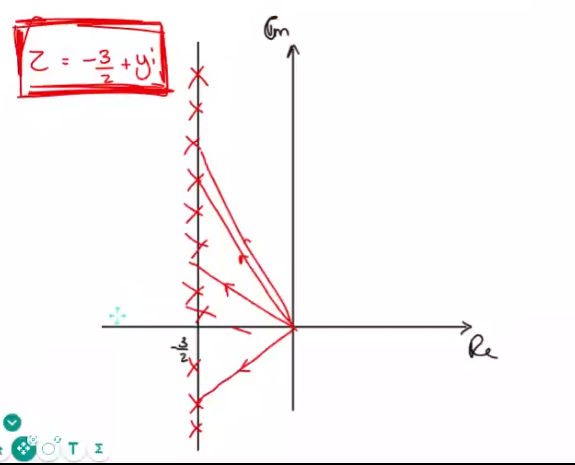
\includegraphics[scale=0.7]{ex1a complex loci}
		\end{center}
	\end{multicols}
	
	\begin{example}
		Given $\abs{\frac{z-1}{z+4i}} = 2 $ , find the locus of $z$.
	\end{example}
	Remembering: $\abs{\frac{z_1}{z_2}} = \frac{\abs{z_1}}{\abs{z_2}}$
	
	
	Let $z = x+yi$
	\begin{alignat*}{2}
		&                & \abs{\frac{z-1}{z+4i}} & = 2                   \\
		& \implies \quad & \abs{z-1}              & = 2\abs{z+4i}         \\
		& \implies \quad & \abs{(x-1)+yi}         & = 2\abs{x+(y+4)i}     \\
		& \implies \quad & \sqrt{(x-1)^2+y^2}     & = 2\sqrt{x^2+(y+4)^2} \\
		& \implies \quad & \sqrt{(x-1)^2+y^2}     & = 2\sqrt{x^2+(y+4)^2} \\
	\end{alignat*}
	\hrulefill
	\begin{example}
		Given that $z_A = \frac{1}{10} (-1+i)$ and $z_B = -\frac{1}{500} (11+127i)$ , find in the form a+bi the complex numbers $\frac{z_A}{z_B}$.
		If $P(x,y)$ is the point on the Argand diagram representing $z=x+yi$, determine the equation of the locus of $P$ where $\abs{z-z_A} = \abs{z-z_B}$.
	\end{example}
	$$\frac{z_A}{z_B}  =  \frac{1}{10} (-1+i) \div -\frac{1}{500} (11+127i)$$
	\begin{alignat*}{2}
		&   &                                     & =-5\cdot \frac{-1+i}{11+127i}                         \\
		&   &                                     & = \frac{5-5i}{11+127i} \cdot  \frac{11-127i}{11-127i} \\
		&   &                                     & = a+bi                                                \\
		&   & \therefore \quad a=-\frac{58}{1625} & ,\quad  b=-\frac{69}{1625}                            \\
		&   & \abs{z-z_A}                         & = \abs{z-z_B}                                         
	\end{alignat*}
	\newpage
	\begin{example}
		If the real part of $\dfrac{z+2}{z+2i}$ is equal to 1, show that the point $z$ lies on a straight line. Hence find the point $z_0$ on this line such that  $\abs{z_0} = \sqrt{2}$. Find also the quadratic equation with real coefficients which has $z_0$ as one of the roots.
	\end{example}
	
	Let $z = x+yi$\\
	\textbf{Showing that $\boldsymbol{z}$ lies on a straight line: }
	\begin{align*}
		&   & Re(\frac{z+2}{z+2i})           & = 1                                                                       \\
		&   & \implies \quad 1               & = Re(\frac{x+2+yi}{x+2i+yi})                                              \\
		&   & \implies \quad 1               & = Re\left(\frac{(x+2)+yi}{x+(y+1)i}\cdot \frac{x-(y+1)i}{x-(y+1)i}\right) \\
		&   & \implies \quad 1               & = Re\left(\frac{x(x+2) -i(y+2)(x+2) + iyx + y(2+y}{x^2 + (y+2)^2}\right)  \\
		&   & \implies \quad 1               & = \frac{x(x+2) + y(y+2)}{x^2 + (y+2)^2}                                   \\
		&   & \implies \quad x(x+2) + y(y+2) & = x^2  + y^2+4y+4                                                         \\
		&   & \implies \quad 2y              & = 2x-4                                                                    \\
	\end{align*}
	$$\therefore \quad y = x-2 \qed$$
	$$\text{Point } z \text{ lies on the straight line } y = x-2$$
	
	\begin{example}
		Shade on an Argand diagram the area represented by $\abs{z+i} < 4$.
	\end{example}~\\
	\setlength{\columnseprule}{0pt}
	\textbf{Finding the loci: }
	\begin{multicols}{2}
		\begin{center}
			\begin{align*}
				&   & \abs{z+i} & = \abs{x+(y+1)i}                                   \\
				&   &           & =\sqrt{x^2  + (y+1)^2}                             \\
				&   &           & =\sqrt{(x-0)^2 + (y-(-1))^2}                       \\
				&   &           & \text{ is the distance from point (0,-1) to (x,y)} 
			\end{align*}
		\end{center}
		\begin{center}
			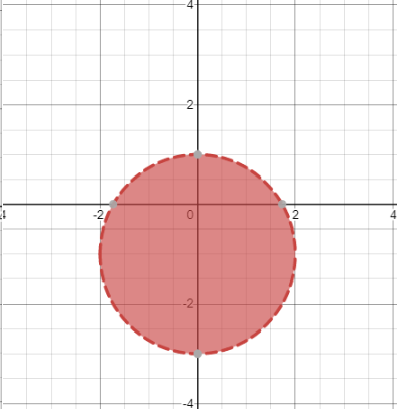
\includegraphics[scale=0.4]{complex_loci_ex5_circle}
		\end{center}
	\end{multicols}


	\textbf{Finding $\boldsymbol{z_0= (a,b) = a+bi\colon}$}
	\reqnomode
	
	\begin{alignat*}{2}
		&               & z_0           & = a+bi           \\
		& \implies      & \abs{z_0}     & = \sqrt{a^2+b^2} \\
		\intertext{Given:  $\abs{z_0}= \sqrt{2}$}
		& \implies\quad & \sqrt{a^+b^2} & = \sqrt{2}       \\
		& \implies\quad & a^2+b^2       & = 2\tag{1}       \\
		\intertext{We also know $z_0$ is on the line $y=x-2$}
		\therefore    b  = a-2\tag{2}	
		\intertext{Substituting 2 in 1: }
		&               & a^2 + (a-2)^2 & = 2              \\
		& \implies\quad & 2a^2 - 4a+4   & = 2              \\
		& \implies\quad & a^2-2a+1      & =0               \\
	\end{alignat*}
	$$	\therefore\quad z_0 = 1-i \qed$$\\
	\textbf{Finding quadratic equation with roots: $\boldsymbol{z_0, \bar{z_0}}$}
	\begin{center}
		$$x^2 - (\text{sum of roots})x + (\text{product of roots}) = 0$$
		$$\implies x^2 - (1-i + 1+i)x + (1-i)(1+i)=0$$
		$$\implies x^2-2x+2 = 0\qed$$
	\end{center}
	
\end{document}